% !TeX program = xelatex
\ifdefined\BookMaster\else
\documentclass[11pt,oneside]{article}
% !TeX program = xelatex
\usepackage[b5paper,left=22mm,right=22mm,top=20mm,bottom=22mm,footskip=11mm]{geometry}
\usepackage{fontspec}
\setmainfont{TeX Gyre Termes}
\setsansfont{TeX Gyre Heros}
\usepackage{amsmath,amssymb,mathtools,amsthm}
\renewcommand{\cdots}{\mathinner{\cdotp\cdotp\cdotp}}
\usepackage{graphicx,adjustbox,array,booktabs,longtable,multirow,enumitem,changepage,needspace}
\usepackage[table]{xcolor}
\usepackage{fancyhdr}
\raggedbottom
\interfootnotelinepenalty=10000
\newcommand{\BookFootnote}[2]{\begingroup\renewcommand{\thefootnote}{\fnsymbol{footnote}}\footnote[#1]{#2}\endgroup}
\newcommand{\BookFootnoteMark}[1]{\begingroup\renewcommand{\thefootnote}{\fnsymbol{footnote}}\footnotemark[#1]\endgroup}
\newcommand{\BookFootnoteText}[2]{\begingroup\renewcommand{\thefootnote}{\fnsymbol{footnote}}\footnotetext[#1]{#2}\endgroup}
\newenvironment{BookFloat}[1]{\par\addvspace{.6\baselineskip}\noindent\def\BookFloatID{#1}\begin{minipage}{\linewidth}\phantomsection\label{bookfloat:#1:start}}{\phantomsection\label{bookfloat:\BookFloatID:end}\end{minipage}\par\addvspace{.6\baselineskip}}

\usepackage[unicode,hidelinks]{hyperref}
\pagestyle{fancy}
\fancyhf{}
\newcommand{\BookFooter}{}
\fancyfoot[L]{\parbox[b]{\dimexpr\textwidth-15mm}{\footnotesize\BookFooter}}
\fancyfoot[R]{\footnotesize\thepage}
\renewcommand{\headrulewidth}{0pt}
\renewcommand{\footrulewidth}{0pt}
\setlength{\parindent}{0pt}
\setlength{\parskip}{0.2em}
\setlength{\emergencystretch}{3em}
\setlist{nosep,leftmargin=1.7em,labelsep=.65em}
\newif\ifBookNarrative
\BookNarrativetrue
\newenvironment{BookBody}{\setlength{\parindent}{0pt}}{}
\newcommand{\BookStatement}[1]{\par\addvspace{.6\baselineskip}\noindent #1\enspace\ignorespaces}
\newcommand{\BookLabel}[1]{\par\addvspace{.6\baselineskip}\needspace{3\baselineskip}\noindent\textbf{#1}\quad\ignorespaces}
\newcommand{\BookHeading}[1]{\par\addvspace{\baselineskip}\needspace{4\baselineskip}\noindent{\large\bfseries #1}\par\medskip}
\newcommand{\BookSubheading}[1]{\par\addvspace{.7\baselineskip}\needspace{3\baselineskip}\noindent{\bfseries #1}\par\smallskip}
\newcommand{\BookTextHeading}[1]{\par\addvspace{.7\baselineskip}\needspace{3\baselineskip}\noindent #1\par\smallskip}
\newcommand{\BookSectionTitle}[2]{\par\addvspace{1.2\baselineskip}\needspace{5\baselineskip}\noindent\colorbox{gray!25}{\sffamily\bfseries\small SECTION #1}\quad{\large\bfseries #2}\par\medskip}
\newcommand{\BookExerciseTitle}[1]{\par\addvspace{\baselineskip}\needspace{4\baselineskip}\noindent{\color{gray}\rule{1.5mm}{1.5mm}}\enspace{\large\bfseries Exercises #1}\par\medskip}
\newcommand{\BookBullet}[1]{\begin{list}{\textbullet}{\setlength{\leftmargin}{1.7em}\setlength{\labelwidth}{1em}\setlength{\labelsep}{.7em}\setlength{\topsep}{0pt}\setlength{\parsep}{0pt}\setlength{\itemsep}{0pt}}\item #1\end{list}}
\newcommand{\BookExercise}[2]{\begin{list}{\textbf{#1}}{\setlength{\leftmargin}{2.2em}\setlength{\labelwidth}{1.5em}\setlength{\labelsep}{.7em}\setlength{\topsep}{.15em}\setlength{\parsep}{0pt}\setlength{\itemsep}{0pt}}\item #2\end{list}}
\newcommand{\BookEnd}[1]{\unskip\nobreak\hfill\ensuremath{#1}}
\newcommand{\BookSource}[2]{\phantomsection\label{sourcepage:#1}} % Source-page anchors, retained through reflow.
\usepackage{multicol}
\usepackage{tikz}
\newcommand{\BookPartEntry}[2]{\par\noindent\makebox[17mm][l]{\bfseries Section #1}#2\par}
\newcommand{\BookPartTitle}[3]{\par\bigskip\noindent\begin{tikzpicture}\node[anchor=north west,inner sep=0pt,outer sep=0pt] (bookpart) at (0,0) {\begin{minipage}{\dimexpr\linewidth-.5pt}\hspace*{26mm}\begin{minipage}[t]{\dimexpr\linewidth-26mm}\begin{adjustbox}{max width=\linewidth}{\fontsize{20}{24}\selectfont\bfseries #2}\end{adjustbox}\par\vspace{6mm}\hrule\vspace{6mm}{\sffamily\footnotesize\setlength{\parskip}{.3em}#3}\vspace{3mm}\end{minipage}\end{minipage}};\path[shade,top color=gray!60,bottom color=white] (0,0) rectangle ([xshift=24mm]bookpart.south west);\node[anchor=north,font=\sffamily\bfseries\small] at (12mm,-2mm) {PART};\node[anchor=north,font=\sffamily\bfseries\Huge] at (12mm,-7mm) {#1};\end{tikzpicture}\par\bigskip}
\newsavebox{\BookMathBox}
\makeatletter
\newcommand{\BookInline}[1]{\leavevmode\hskip0pt\relax\begingroup\in@{\begin}{#1}\ifin@\sbox{\BookMathBox}{\(#1\)}\ifdim\wd\BookMathBox>\dimexpr\linewidth-1em\relax\resizebox{\dimexpr\linewidth-1em\relax}{!}{\usebox{\BookMathBox}}\else\(#1\)\fi\else\in@{\left}{#1}\ifin@\sbox{\BookMathBox}{\(#1\)}\ifdim\wd\BookMathBox>\dimexpr\linewidth-1em\relax\resizebox{\dimexpr\linewidth-1em\relax}{!}{\usebox{\BookMathBox}}\else\(#1\)\fi\else\(#1\)\fi\fi\endgroup\hskip0pt\relax}
\makeatother
\DeclareMathOperator{\Aut}{Aut}
\DeclareMathOperator{\End}{End}
\DeclareMathOperator{\Hom}{Hom}
\DeclareMathOperator{\GF}{GF}
\DeclareMathOperator{\irr}{irr}
\DeclareMathOperator{\lt}{lt}
\DeclareMathOperator{\lp}{lp}
\providecommand{\textcircled}[1]{\textnormal{(#1)}}

\begin{document}
\fi
\renewcommand{\BookFooter}{Section 46 Galois Theory}
\pdfbookmark[0]{Section 46 Galois Theory}{46_galois_theory}
\ifdefined\BookMaster\else\setcounter{page}{364}\fi
% Source PDF page 381; original printed page 364
\BookSource{381}{364}
\BookNarrativetrue

\begin{BookBody}

\BookSectionTitle{46}{Galois Theory}

\BookTextHeading{\textbf{The Galois Theorems}  }

\noindent In this section we present the main theorems of Galois theory. These theorems provide precise statements regarding the correspondence between intermediate fields of a normal field extension and subgroups of the Galois group. But first we state key definitions related to the correspondence.

\BookLabel{46.1 Definition} Let \BookInline{K} be a normal extension of \BookInline{F,\allowbreak E} an intermediate field of the extension, and \BookInline{H} a subgroup of \BookInline{G(K/F).} The set of all \BookInline{\alpha \in K} such that each element of \BookInline{H} fixes \BookInline{\alpha } is an 
% Source PDF page 382; original printed page 365
\BookSource{382}{365}
intermediate field of the extension \BookInline{K} over \BookInline{F,\allowbreak } and it is called the\textbf{ fixed field for} \BookInline{H.} We write \BookInline{K_{H}} to denote the fixed field for \BookInline{H.}

\end{BookBody}

\BookNarrativetrue

\begin{BookBody}

We let \BookInline{\lambda (E)} be the set of all \BookInline{\sigma \in G(K/F)} that fix all the elements of \BookInline{E,\allowbreak } that is, \BookInline{\lambda (E)= G(K/E).} We call \BookInline{\lambda (E)} the\textbf{ group of} \BookInline{E.}

If \BookInline{K} is the splitting field of \BookInline{f(x)\in F[x],\allowbreak } then we say that \BookInline{G(K/F)} is the\textbf{ group of} \textbf{the polynomial} \BookInline{f(x).}\BookEnd{\blacksquare}

\BookLabel{46.2 Example} Let \BookInline{K} be the splitting field of \BookInline{f(x)= x^{3}- 2} over \BookInline{\mathbb{Q}.} As we saw in Example \BookInline{45.19,\allowbreak K} is a normal extension of \BookInline{\mathbb{Q}} and

\begin{center}\begin{adjustbox}{max width=\linewidth}\BookInline{\displaystyle K = \mathbb { Q } ( { \sqrt [ 3 ] { 2 } } ,\allowbreak  { \sqrt { 3 } } i ) .}\end{adjustbox}\end{center}

\noindent The group of \BookInline{f(x)} is \BookInline{G(K/\mathbb{Q}).} Also,

\begin{center}\begin{adjustbox}{max width=\linewidth}\BookInline{\displaystyle \lambda ( \mathbb { Q } ( { \sqrt [ 3 ] { 2 } } ) ) = \{ \sigma \in G ( K / \mathbb { Q } )   |   \sigma ( { \sqrt [ 3 ] { 2 } } ) = { \sqrt [ 3 ] { 2 } } \} = G ( K / \mathbb { Q } ( { \sqrt [ 3 ] { 2 } } ) ) .}\end{adjustbox}\end{center}

Both the identity\BookInline{,\allowbreak \iota,\allowbreak } and complex conjugation\BookInline{,\allowbreak \sigma (a+ } \textit{bi}\BookInline{)\; = a- } \textit{bi}, fix \BookInline{{ \sqrt { 2 } }.} Therefore,

\begin{center}\begin{adjustbox}{max width=\linewidth}\BookInline{\displaystyle \langle \sigma \rangle = \{ \iota ,\allowbreak  \sigma \} \leq \lambda ( \mathbb { Q } ( { \sqrt [ 3 ] { 2 } } ) )}\end{adjustbox}\end{center}

\noindent and

\begin{center}\begin{adjustbox}{max width=\linewidth}\BookInline{\displaystyle K _ { \sigma } = \mathbb { Q } ( { \sqrt [ 3 ] { 2 } } ) .}\end{adjustbox}\end{center}

At this point, we can only say \BookInline{\langle \sigma \rangle } is a subgroup of \BookInline{\lambda ( \mathbb { Q } ( { \sqrt [ 3 ] { 2 } } ) )} since it is conceivable that there could be other automorphisms of \BookInline{G(K/\mathbb{Q})} that fix \BookInline{\mathbb { Q } ( { \sqrt [ 3 ] { 2 } } )}. As we will soon see, this cannot be the case, and the two subgroups are equal\BookInline{.}\BookEnd{\blacktriangle}

We now present a series of related theorems that together make up the essence of Galois Theory.

\BookLabel{46.3 Theorem} Let \BookInline{K} be a normal extension of a field \BookInline{F} and \BookInline{E} an intermediate field. The fixed field for the set of all automorphisms of \BookInline{K} that fix \BookInline{E} is exactly \BookInline{E.} That is,

\begin{center}\begin{adjustbox}{max width=\linewidth}\BookInline{\displaystyle E= K_{\lambda (E)}.}\end{adjustbox}\end{center}

\BookLabel{\textit{Proof}} Clearly \BookInline{E\subseteq K_{\lambda (E)}.} We show that \BookInline{K_{\lambda (E)}\subseteq E.} Let \BookInline{\alpha } be an element of \BookInline{K} that is not in \BookInline{E.} The minimal polynomial for \BookInline{\alpha } over \BookInline{E} has degree at least two and therefore \BookInline{\alpha } has a conjugate \BookInline{\beta \in K,\allowbreak } with \BookInline{\beta \neq \alpha,\allowbreak } by Corollary 44.12 and the fact that \BookInline{K} is a separable extension of \BookInline{F.} Theorem 43.18, the Conjugation Isomorphism Theorem, says there is an isomorphism

\begin{center}\begin{adjustbox}{max width=\linewidth}\BookInline{\displaystyle \psi _{\alpha ,\allowbreak \beta }:E(\alpha )\to E(\beta )}\end{adjustbox}\end{center}

\noindent that maps \BookInline{\alpha } to \BookInline{\beta } and fixes all the elements of \BookInline{E.} The map \BookInline{\psi _{\alpha,\allowbreak \beta }} can be extended to an automorphism \BookInline{\sigma:K\to K} by the Isomorphism Extension Theorem, Theorem 44.6. Thus \BookInline{\sigma \in \lambda (E),\allowbreak } and \BookInline{\sigma } does not fix \BookInline{\alpha.} We have shown that if \BookInline{\alpha \notin E,\allowbreak } then \BookInline{\lambda (E)} does not fix \BookInline{\alpha;} or equivalently\BookInline{,\allowbreak K_{\lambda (E)}\subseteq E,\allowbreak } which completes the proof\BookInline{.}\BookEnd{\blacklozenge}

\BookLabel{46.4 Theorem} Let \BookInline{K} be a normal extension of a field \BookInline{F} and \BookInline{E} an intermediate field. The degree of the extension \BookInline{K} over \BookInline{E} is the order of the group \BookInline{\lambda (E):}

\begin{center}\begin{adjustbox}{max width=\linewidth}\BookInline{\displaystyle [K:E]= |\lambda (E)|= |G(K/E)|.}\end{adjustbox}\end{center}

\noindent Furthermore, the number of left cosets of \BookInline{\lambda (E)} in \BookInline{G(K/F)} is the degree of the extension of \BookInline{E} over \BookInline{F.} That is,

\begin{center}\begin{adjustbox}{max width=\linewidth}\BookInline{\displaystyle (G(K/F):\lambda (E))= [E:F].}\end{adjustbox}\end{center}

\BookLabel{\textit{Proof}} Since \BookInline{\lambda (E)= G(K/E),\allowbreak } this theorem is simply a restatement of Corollary \BookInline{45.18.}\BookEnd{\blacklozenge}

\end{BookBody}

% Source PDF page 383; original printed page 366
\BookSource{383}{366}
\BookNarrativetrue

\begin{BookBody}

\BookLabel{46.5 Example} Continuing Example 46.2, \BookInline{K = \mathbb { Q } ( { \sqrt [ 3 ] { 2 } },\allowbreak { \sqrt { 3 } } i )} is the splitting field of \BookInline{x^{3}- 2} over \BookInline{\mathbb{Q}.} We saw that if \BookInline{\sigma } is complex conjugation, then \BookInline{\langle \sigma \rangle \leq \lambda ( \mathbb { Q } ( { \sqrt [ 3 ] { 2 } } ) )}. The degree of the extension \BookInline{K} over \BookInline{\mathbb { Q } ( { \sqrt [ 3 ] { 2 } } )} is two since \BookInline{\alpha = \sqrt{3}i\notin K,\allowbreak } but \BookInline{\alpha } is a zero of the degree 2 polynomial \BookInline{x ^ { 2 } + 3 \in \mathbb { Q } ( { \sqrt [ 3 ] { 2 } } ) [ x ]}. By Theorem 46.4,

\begin{center}\begin{adjustbox}{max width=\linewidth}\BookInline{\displaystyle 2 = [ K : \mathbb { Q } ( { \sqrt [ 3 ] { 2 } } ) ] = | \lambda ( \mathbb { Q } ( { \sqrt [ 3 ] { 2 } } ) ) | .}\end{adjustbox}\end{center}

Since \BookInline{\langle \sigma \rangle \leq \lambda ( \mathbb { Q } ( { \sqrt [ 3 ] { 2 } } ) )} and both finite groups have the same number of elements,

\begin{center}\begin{adjustbox}{max width=\linewidth}\BookInline{\displaystyle \langle \sigma \rangle = \lambda ( \mathbb { Q } ( { \sqrt [ 3 ] { 2 } } ) ) .}\end{adjustbox}\end{center} \BookEnd{\blacktriangle}

\BookLabel{46.6 Theorem} Let \BookInline{K} be a normal extension of a field \BookInline{F} and \BookInline{H} a subgroup of the Galois group \BookInline{G(K/F).} The subgroup of \BookInline{G(K/F)} that fixes all the elements fixed by \BookInline{K_{H}} is exactly \BookInline{H.} That is,

\begin{center}\begin{adjustbox}{max width=\linewidth}\BookInline{\displaystyle \lambda (K_{H})= H.}\end{adjustbox}\end{center}

\BookLabel{\textit{Proof}} It is clear that \BookInline{H} is a subgroup of \BookInline{\lambda (K_{H}).} We will verify that the two groups are equal by checking that they have the same number of elements. Let \BookInline{k= |H|.}

By Theorem 45.13, the field extension \BookInline{K} over \BookInline{F} has a primitive element\BookInline{,\allowbreak \alpha,\allowbreak } so \BookInline{K= F(\alpha ).} Let \BookInline{E= K_{H},\allowbreak } the subfield of \BookInline{K} that is fixed by every element in \BookInline{H.} Then \BookInline{K= E(\alpha )} and \BookInline{[K:E]= } deg\BookInline{(\alpha,\allowbreak E).} We let \BookInline{n= [K:E].} We next let

\begin{center}\begin{adjustbox}{max width=\linewidth}\BookInline{\displaystyle f(x)= _{\sigma }\prod _{\in H}(x- \sigma (\alpha ))\in K[x].}\end{adjustbox}\end{center}

\noindent The degree of \BookInline{f} is \BookInline{k= |H|.} Let \BookInline{\tau \in H,\allowbreak } so \BookInline{\tau } is an isomorphism from \BookInline{K} onto \BookInline{K.} Since \BookInline{H} is a group, multiplying all the elements of \BookInline{H} by \BookInline{\tau } on the left simply permutes the elements of \BookInline{H.} That is,

\begin{center}\begin{adjustbox}{max width=\linewidth}\BookInline{\displaystyle H= \{\sigma _{1},\allowbreak \sigma _{2},\allowbreak ...,\allowbreak \sigma _{k}\}= \{\tau \sigma _{1},\allowbreak \tau \sigma _{2},\allowbreak ...,\allowbreak \tau \sigma _{k}\}.}\end{adjustbox}\end{center}

\noindent By Exercise 32 in Section 44, the map \BookInline{\tau _{x}:K[x]\to K[x]} is an isomorphism and

\begin{center}\begin{adjustbox}{max width=\linewidth}\BookInline{\displaystyle \tau _{x}(f(x))= _{\sigma }\prod _{\in H}(x- \tau \sigma (\alpha ))= _{\sigma }\prod _{\in H}(x- \sigma (\alpha ))= f(x).}\end{adjustbox}\end{center}

\noindent Writing \BookInline{f(x)= a_{0}+ a_{1}x+ a_{2}x^{2}+ \cdots + a_{k}x^{k},\allowbreak }

\begin{center}\begin{adjustbox}{max width=\linewidth}\BookInline{\displaystyle \tau _{x}(f(x))= \tau (a_{0})+ \tau (a_{1})x+ \tau (a_{2})x^{2}+ \cdots + \tau (a_{k})x^{k}.}\end{adjustbox}\end{center}

\noindent Equating coefficients in \BookInline{\tau _{x}(f(x))= f(x),\allowbreak } we see that for any \BookInline{\tau \in H,\allowbreak } and for any \BookInline{i,\allowbreak a_{i}= } \BookInline{\tau (a_{i}).} But the only elements of \BookInline{K} that are fixed by every element in \BookInline{H} are the elements of \BookInline{E= K_{H},\allowbreak } which implies that each \BookInline{a_{i}} is in \BookInline{E.} Therefore\BookInline{,\allowbreak f(x)\in E[x].} Since the identity map is in \BookInline{H,\allowbreak \alpha } is a zero of \BookInline{f(x).} Thus irr\BookInline{(\alpha,\allowbreak E)} divides \BookInline{f(x)} and

\begin{center}\begin{adjustbox}{max width=\linewidth}\BookInline{\displaystyle k= \;\text{deg}\;(f(x))\geq \;\text{deg}\;(\;\text{irr}\;(\alpha ,\allowbreak E))= \;\text{deg}\;(\alpha ,\allowbreak E)= n.}\end{adjustbox}\end{center}

\noindent Since \BookInline{H} is a subgroup of \BookInline{\lambda (K_{H}),\allowbreak }

\begin{center}\begin{adjustbox}{max width=\linewidth}\BookInline{\displaystyle k= |H|\leq |\lambda (K_{H})|= [K:E]= n.}\end{adjustbox}\end{center}

\noindent Thus we have \BookInline{k= n} and \BookInline{\lambda (K_{H})= H.} \BookEnd{\blacklozenge}

Theorems 46.3 and 46.6 together imply that for normal extensions, the map \BookInline{\lambda,\allowbreak } which maps the intermediate fields of the extension \BookInline{K} over \BookInline{F} to subgroups of \BookInline{G(K/F),\allowbreak } is both one-to-one and onto. Furthermore the inverse map \BookInline{\lambda ^{- 1}} is simply the map that sends a subgroup \BookInline{H\leq G(K/E)} to the intermediate field \BookInline{K_{H}= G(K/E).}

\BookLabel{46.7 Example} Let \BookInline{K = \mathbb { Q } ( { \sqrt [ 3 ] { 2 } },\allowbreak { \sqrt { 3 } } i )} over \BookInline{\mathbb{Q}.} In Example 45.19, we determined that \BookInline{|G(K/\mathbb{Q})|= 6.} In this example, we take an alternate route to arrive at the same conclusion. In

\end{BookBody}

% Source PDF page 384; original printed page 367
\BookSource{384}{367}
\BookNarrativetrue

\begin{BookBody}

Example 46.5, we saw that for \BookInline{\sigma \in G(K/\mathbb{Q})} given by complex conjugation, \BookInline{\lambda(\mathbb{Q}(\sqrt[3]{2})) =} \BookInline{\langle \sigma \rangle.} Therefore,

\begin{center}\begin{adjustbox}{max width=\linewidth}\BookInline{\displaystyle K _ { \langle \sigma \rangle } = \mathbb { Q } ( { \sqrt [ 3 ] { 2 } } ) .}\end{adjustbox}\end{center}

Theorem 46.4 says that

\begin{center}\begin{adjustbox}{max width=\linewidth}\BookInline{\displaystyle ( G ( K / \mathbb { Q } ) : \langle \sigma \rangle ) = ( G ( K / \mathbb { Q } ) : \lambda ( \mathbb { Q } ( { \sqrt [ 3 ] { 2 } } ) ) = [ \mathbb { Q } ( { \sqrt [ 3 ] { 2 } } : \mathbb { Q } ] = 3 .}\end{adjustbox}\end{center}

\noindent Since \BookInline{|\langle \sigma \rangle |= 2,\allowbreak }

\begin{center}\begin{adjustbox}{max width=\linewidth}\BookInline{\displaystyle |G(K/\mathbb{Q})|= (G(K/\mathbb{Q}):\langle \sigma \rangle )\cdot |\langle \sigma \rangle |= 6.}\end{adjustbox}\end{center} \BookEnd{\blacktriangle}

\BookLabel{46.8 Theorem} Let \BookInline{K} be a normal extension of a field \BookInline{F} and \BookInline{E} an intermediate field of the extension. Then \BookInline{E} is a normal extension of \BookInline{F} if and only if \BookInline{\lambda (E)} is a normal subgroup of \BookInline{G(K/F).} Furthermore, if \BookInline{E} is a normal extension of \BookInline{F,\allowbreak } then \BookInline{G(E/F)} is isomorphic with \BookInline{G(K/F)/G(K/E).}

\BookLabel{\textit{Proof}} We first assume that \BookInline{E} is a normal extension of \BookInline{F.} Let \BookInline{\tau \in \lambda (E)= G(K/E)} and \BookInline{\sigma \in } \BookInline{G(K/F).} We verify that \BookInline{\sigma \tau \sigma ^{- 1}\in G(K/E)} to show that \BookInline{\lambda (E)} is a normal subgroup of \BookInline{G(K/F).} By Theorem \BookInline{44.11,\allowbreak \sigma ^{- 1}} maps \BookInline{E} isomorphically onto \BookInline{E.} Therefore, for any \BookInline{\alpha \in E,\allowbreak \tau (\sigma ^{- 1}(\alpha ))= \sigma ^{- 1}(\alpha )} and

\begin{center}\begin{adjustbox}{max width=\linewidth}\BookInline{\displaystyle \sigma \tau \sigma ^{- 1}(\alpha )= \sigma (\tau (\sigma ^{- 1}(\alpha )))= \sigma (\sigma ^{- 1}(\alpha ))= \alpha .}\end{adjustbox}\end{center}

\noindent Thus\BookInline{,\allowbreak \sigma \tau \sigma ^{- 1}\in G(K/E),\allowbreak } and \BookInline{\lambda (E)} is a normal subgroup of \BookInline{G(K/F).}

We next assume that \BookInline{\lambda (E)} is a normal subgroup of \BookInline{G(K/F)} and show that \BookInline{E} is a normal extension of \BookInline{F.} We must show that \BookInline{E} is a splitting field over \BookInline{F} and that \BookInline{E} is a separable extension of \BookInline{F.} Theorem 45.8 says that the extension is separable. We use Corollary 44.14 to show that \BookInline{E} is a splitting field over \BookInline{F.} Let \BookInline{\sigma _{1}} be any isomorphism fixing \BookInline{F} and mapping \BookInline{E} onto a subfield of \BookInline{K.} Let \BookInline{\sigma } be an extension of \BookInline{\sigma _{1}} to an isomorphism from \BookInline{K} onto \BookInline{K.} Such an extension exists by the Isomorphism Extension Theorem 44.6. Let \BookInline{\alpha \in E} and \BookInline{\tau \in \lambda (E).} By assumption \BookInline{\sigma ^{- 1}\tau \sigma (\alpha )= \alpha.} Thus

\begin{center}\begin{adjustbox}{max width=\linewidth}\BookInline{\displaystyle \tau \sigma (\alpha )= \sigma (\alpha ).}\end{adjustbox}\end{center}

\noindent Since every \BookInline{\tau \in \lambda (E)} fixes \BookInline{\sigma (\alpha ),\allowbreak \sigma (\alpha )\in K_{\lambda (E)}.} By Theorem \BookInline{46.3,\allowbreak \sigma (\alpha )\in E.} Thus the isomorphism \BookInline{\sigma _{1}} maps \BookInline{E} isomorphically onto \BookInline{E.} By Corollary \BookInline{44.14,\allowbreak E} is a splitting field over \BookInline{F,\allowbreak } and therefore\BookInline{,\allowbreak E} is a normal extension of \BookInline{F.}

Assuming that \BookInline{E} is a normal extension of \BookInline{F,\allowbreak } we know that any isomorphism of \BookInline{K} that fixes \BookInline{F} maps \BookInline{E} isomorphically onto itself. Using this fact, we can define \BookInline{\phi:G(K/F)\to G(E/F)} by simply letting \BookInline{\phi (\sigma )} be the map \BookInline{\sigma } restricted to \BookInline{E.} By the Isomorphism Extension Theorem \BookInline{44.6,\allowbreak \phi } maps onto \BookInline{G(E/F).} Also

\begin{center}\begin{adjustbox}{max width=\linewidth}\BookInline{\displaystyle \;\text{Ker}\;(\phi )= \{\sigma \in G(K/F)\mid \sigma (\alpha )= \alpha \;\text{for all}\;\alpha \in E\}= G(K/E).}\end{adjustbox}\end{center}

\noindent Therefore \BookInline{G(E/F)} is isomorphic with

\begin{center}\begin{adjustbox}{max width=\linewidth}\BookInline{\displaystyle G(K/F)/\;\text{Ker}\;(\phi )= G(K/F)/G(K/E).}\end{adjustbox}\end{center} \BookEnd{\blacklozenge}

\BookLabel{46.9 Example} Recall from Example \BookInline{43.14,\allowbreak x^{3}- 2} has only one zero in the field extension \BookInline{\mathbb { Q } ( { \sqrt [ 3 ] { 2 } } )} over \BookInline{\mathbb{Q}.} Thus \BookInline{\mathbb { Q } ( { \sqrt [ 3 ] { 2 } } )} over \BookInline{\mathbb{Q}} is not a splitting field, and therefore, not a normal extension. As we saw, the only automorphism of \BookInline{G ( \mathbb { Q } ( { \sqrt [ 3 ] { 2 } } ) / \mathbb { Q } )} is the identity map \BookInline{\iota.} So the set of automorphisms of \BookInline{\mathbb { Q } ( { \sqrt [ 3 ] { 2 } } )} fixing \BookInline{\mathbb { Q } ( { \sqrt [ 3 ] { 2 } } )} is the same as the set of automorphisms of \BookInline{\mathbb { Q } ( { \sqrt [ 3 ] { 2 } } )} fixing \BookInline{\mathbb{Q}.} In the case of a normal extension, this could not happen since \BookInline{\lambda } gives a one-to-one correspondence.

In Example 46.7, we saw that

\begin{center}\begin{adjustbox}{max width=\linewidth}\BookInline{\displaystyle | G ( \mathbb { Q } ( { \sqrt [ 3 ] { 2 } } ,\allowbreak  { \sqrt { 3 } } i ) / \mathbb { Q } ) | = 6 .}\end{adjustbox}\end{center}

\end{BookBody}

% Source PDF page 385; original printed page 368
\BookSource{385}{368}
\BookNarrativetrue

\begin{BookBody}

Up to isomorphism, there are only two groups of order \BookInline{6,\allowbreak \mathbb{Z}_{6}} and \BookInline{S_{3}.} Since \BookInline{\mathbb { Q } ( { \sqrt [ 3 ] { 2 } } )} over \BookInline{\mathbb{Q}} is not a normal extension of \BookInline{\widetilde{\mathbb{Q}},\allowbreak \lambda(\mathbb{Q}(\sqrt[3]{2}))} is not a normal subgroup of \BookInline{G ( \mathbb { Q } ( { \sqrt [ 3 ] { 2 } },\allowbreak { \sqrt { 3 } } i ) / \mathbb { Q } )}. Every subgroup of \BookInline{\mathbb{Z}_{6}} is a normal subgroup, so \BookInline{G ( \mathbb { Q } ( { \sqrt [ 3 ] { 2 } },\allowbreak { \sqrt [ 3 ] { 3 } } i ) / \mathbb { Q } )} is isomorphic with \BookInline{S_{3}.}\BookEnd{\blacktriangle}

The next theorem completes the basic facts that are used to apply Galois theory to particular problems. The theorem is usually interpreted in terms of subgroup and subfield diagrams. It says that the diagram for subfields is the same as the diagram for the corresponding subgroups, except that the diagrams are inverted.

\BookLabel{46.10 Theorem} Let \BookInline{K} be a normal extension of \BookInline{F,\allowbreak } with \BookInline{E_{1}} and \BookInline{E_{2}} intermediate fields. Then

\BookInline{E_{1}} is a subfield of \BookInline{E_{2}} if and only if \BookInline{\lambda (E_{2})} is a subgroup of \BookInline{\lambda (E_{1}).}

\BookLabel{\textit{Proof}} Suppose that \BookInline{E_{1}\leq E_{2}.} Then any automorphism of \BookInline{K} that fixes every element of \BookInline{E_{2}} clearly fixes every element of \BookInline{E_{1},\allowbreak } which means that \BookInline{\lambda (E_{2})\leq \lambda (E_{1}).}

Now suppose that \BookInline{\lambda (E_{2})\leq \lambda (E_{1}).} Let \BookInline{\alpha \in K_{\lambda (E_{1})}}. Then \BookInline{\alpha } is fixed by every element of \BookInline{\lambda (E_{1})} and, therefore, by every element of \BookInline{\lambda (E_{2}).} So \BookInline{\alpha \in K_{\lambda (E_{2})}}. Thus

\begin{center}\begin{adjustbox}{max width=\linewidth}\BookInline{\displaystyle E_{1}= K_{\lambda (E_{1})}\leq K_{\lambda (E_{2})}= E_{2}.}\end{adjustbox}\end{center} \BookEnd{\blacklozenge}

\BookLabel{46.11 Example} As before, we let \BookInline{K} be the splitting field for \BookInline{f(x)= x^{3}- 2} over \BookInline{\mathbb{Q}.} Each \BookInline{\sigma \in G(K/\mathbb{Q})} is completely determined by how \BookInline{\sigma } permutes the zeros of \BookInline{f(x).} Since \BookInline{f(x)} has three zeros\BookInline{,\allowbreak G(K/E)} is isomorphic with a subgroup of the symmetric group \BookInline{S_{3}.} As we saw in Example \BookInline{46.9,\allowbreak G(K/\mathbb{Q})} is isomorphic with \BookInline{S_{3}.} By labeling the zeros of \BookInline{f(x)} by

\begin{center}\begin{adjustbox}{max width=\linewidth}\BookInline{\displaystyle \begin{aligned} &r_{1} = \sqrt[3]{2} \\&r_{2} = \frac{\sqrt[3]{2}}{2} \left( - 1 + \sqrt{3}i \right) \\&r_{3} = \frac{\sqrt[3]{2}}{2} \left( - 1 - \sqrt{3}i \right)\\ \end{aligned}}\end{adjustbox}\end{center}

\noindent the isomorphism \BookInline{\phi:G(K/\mathbb{Q})\to S_{3}} can be defined by letting \BookInline{\phi (\sigma )} be the permutation of the zeros of \BookInline{f(x)} by the automorphism \BookInline{\sigma,\allowbreak } that is\BookInline{,\allowbreak \phi (\sigma )(i)= j} if \BookInline{\sigma (r_{i})= r_{j}.} We will abuse notation slightly and identify elements in \BookInline{G(K/\mathbb{Q})} with their corresponding elements in the symmetric group \BookInline{S_{3}.}

The subgroup diagram for \BookInline{S_{3}} is displayed in Figure 46.12 (a). By Theorem 46.10, the subfield diagram for \BookInline{K} is given in Figure 46.12 (b).

The automorphism corresponding to the transposition (2, 3) maps \BookInline{r_{2}} to \BookInline{r_{3},\allowbreak } maps \BookInline{r_{3}} to \BookInline{r_{2},\allowbreak } and fixes \BookInline{r_{1},\allowbreak } which is complex conjugation. As we saw in Example \BookInline{46.7,\allowbreak K_{\langle (2,\allowbreak 3)\rangle }= } \BookInline{\mathbb { Q } ( { \sqrt [ 3 ] { 2 } } ) = \mathbb { Q } ( r _ { 1 } )}. The automorphism corresponding to (1, 2) fixes \BookInline{r_{3},\allowbreak } maps \BookInline{r_{1}} to \BookInline{r_{2},\allowbreak } and maps \BookInline{r_{2}} to \BookInline{r_{1}.} Thus \BookInline{K_{\langle (1,\allowbreak 2)\rangle }= \mathbb{Q}(r_{3}).} Similarly\BookInline{,\allowbreak K_{\langle (1,\allowbreak 3)\rangle }= \mathbb{Q}(r_{2}).}

We can determine \BookInline{K_{\langle (1,\allowbreak 2,\allowbreak 3)\rangle }} by noticing that

\begin{center}\begin{adjustbox}{max width=\linewidth}\BookInline{\displaystyle \begin{aligned} | \lambda ( \mathbb { Q } ( \sqrt { 3 } i ) ) | &= [ K : \mathbb { Q } ( \sqrt { 3 } i ) ] \\&= [ \mathbb { Q } ( \sqrt [ 3 ] { 2 } ,\allowbreak  \sqrt { 3 } i ) : \mathbb { Q } ( \sqrt { 3 } i ) ] \\&= [ \mathbb { Q } ( \sqrt [ 3 ] { 2 } ,\allowbreak  \sqrt { 3 } i ) : \mathbb { Q } ) ] / [ \mathbb { Q } ( \sqrt { 3 } i ) : \mathbb { Q } ] \\&= 3.\\ \end{aligned}}\end{adjustbox}\end{center}

\noindent The subfield diagram shows that there is only one intermediate field \BookInline{E} with \BookInline{[K:E]= 3,\allowbreak } so \BookInline{K_{\langle (1,\allowbreak 2,\allowbreak 3)\rangle }= \mathbb{Q}(\sqrt{3}i).} Summarizing:

\begin{center}\begin{adjustbox}{max width=\linewidth}\BookInline{\displaystyle \begin{aligned}K_{\{\iota\}} &= K \\K_{S_{3}} &= \mathbb{Q} \\K_{\iota} &= \mathbb{Q}(r_{\iota}) = \mathbb{Q}(\sqrt[3]{2})\end{aligned}}\end{adjustbox}\end{center}

\end{BookBody}

% Source PDF page 386; original printed page 369
\BookSource{386}{369}
\BookNarrativetrue

\begin{BookBody}

\begin{BookFloat}{46_galois_theory-p386-0}
\begin{center}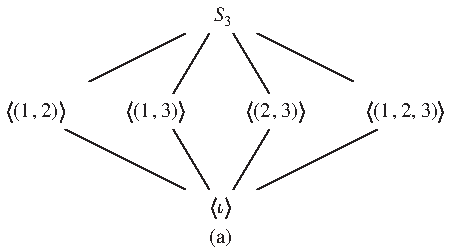
\includegraphics[width=0.616\linewidth,height=.8\textheight,keepaspectratio]{assets/p386_00.pdf}\end{center}
\end{BookFloat}

\begin{BookFloat}{46_galois_theory-p386-1}
\begin{center}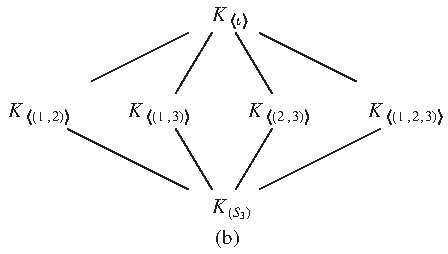
\includegraphics[width=0.614\linewidth,height=.8\textheight,keepaspectratio]{assets/p386_01.pdf}\end{center}
\begin{center}\small\textbf{46.12 Figure}\end{center}
\end{BookFloat}

\begin{center}\begin{adjustbox}{max width=\linewidth}\BookInline{\displaystyle K _ { \langle ( 1 ,\allowbreak  2 ) \rangle } = \mathbb { Q } ( r _ { 3 } ) = \mathbb { Q } \left( \frac { \sqrt [ 3 ] { 2 } } { 2 } \left( - 1 - \sqrt { 3 } i \right) \right)}\end{adjustbox}\end{center}

\begin{center}\begin{adjustbox}{max width=\linewidth}\BookInline{\displaystyle K _ { \langle ( 1 ,\allowbreak  3 ) \rangle } = \mathbb { Q } ( r _ { 2 } ) = \mathbb { Q } \left( \frac { \sqrt [ 3 ] { 2 } } { 2 } \left( - 1 + \sqrt { 3 } i \right) \right)}\end{adjustbox}\end{center}

\begin{center}\begin{adjustbox}{max width=\linewidth}\BookInline{\displaystyle K_{\langle (1,\allowbreak 2,\allowbreak 3)\rangle }= \mathbb{Q}(\sqrt{3}i)}\end{adjustbox}\end{center}

Normal subgroups of \BookInline{G(K/\mathbb{Q})} correspond to subfields of \BookInline{K} that are normal extensions of \BookInline{\mathbb{Q}} by Theorem 46.8. Thus the only intermediate fields of \BookInline{K} that are normal extensions of \BookInline{\mathbb{Q}} are \BookInline{K,\allowbreak \mathbb{Q},\allowbreak } and \BookInline{\mathbb{Q}(\sqrt{3}i)} corresponding to the normal subgroups of \BookInline{S_{3},\allowbreak } namely \BookInline{\{\iota \},\allowbreak S_{3},\allowbreak } and \BookInline{\langle (1,\allowbreak 2,\allowbreak 3)\rangle,\allowbreak } respectively\BookInline{.}\BookEnd{\blacktriangle}

Not every subgroup diagram of a Galois group looks like its own inversion, as we will see in the next section. \BookEnd{\blacksquare}

\end{BookBody}

\BookNarrativefalse

\begin{BookBody}

\BookExerciseTitle{46}

\BookTextHeading{\textbf{Computations}}

\noindent The field \BookInline{K= \mathbb{Q}(\sqrt{2},\allowbreak \sqrt{3},\allowbreak \sqrt{5})} is a finite normal extension of \BookInline{\mathbb{Q}.} It can be shown that \BookInline{[K:\mathbb{Q}]= 8.} In Exercises 1 through 8, compute the indicated numerical quantity. The notation is that of Definition 46.1.

\BookExercise{2.}{\BookInline{|G(K/\mathbb{Q})|}}

\BookExercise{1.}{\BookInline{[K:\mathbb{Q}\sqrt{2}]}}

\BookExercise{4.}{\BookInline{|\lambda (\mathbb{Q}(\sqrt{2},\allowbreak \sqrt{3}))|}}

\BookExercise{3.}{\BookInline{|\lambda (\mathbb{Q})|}}

\BookExercise{6.}{\BookInline{|\lambda (\mathbb{Q}(\sqrt{30}))|}}

\BookExercise{5.}{\BookInline{|\lambda (\mathbb{Q}(\sqrt{6}))|}}

\BookExercise{8.}{\BookInline{|\lambda (K)|}}

\BookExercise{7.}{\BookInline{|\lambda (\mathbb{Q}(\sqrt{2}+ \sqrt{6}))|}}

\end{BookBody}

% Source PDF page 387; original printed page 370
\BookSource{387}{370}
\BookNarrativefalse

\begin{BookBody}

\BookExercise{9.}{Describe the group of the polynomial \BookInline{(x^{4}- 1)\in \mathbb{Q}[x]} over \BookInline{\mathbb{Q}.}}

\BookExercise{10.}{Let \BookInline{G} be the group of the polynomial \BookInline{x^{3}+ 2} over \BookInline{\mathbb{Q}.} Find the order of \BookInline{G} and identify a well-known group that is isomorphic with \BookInline{G.}}

\BookExercise{11.}{Let \BookInline{K} be the splitting field of \BookInline{x^{3}- 5} over \BookInline{\mathbb{Q}.}}

\textbf{a.} Show that \BookInline{K= \mathbb{Q}(\sqrt[3]{5},\allowbreak i\sqrt{3}).}

\textbf{b.} Describe the six elements of \BookInline{G(K/\mathbb{Q})} by giving their values on \BookInline{\sqrt { 5 }} and \BookInline{i\sqrt{3}.}

\BookExercise{c.}{To what group we have seen before is \BookInline{G(K/\mathbb{Q})} isomorphic?}

\BookExercise{d.}{Using the notation given in the answer to part (b) in the back of the text, give the diagrams for the subfields of \BookInline{K} and for the subgroups of \BookInline{G(K/\mathbb{Q}),\allowbreak } indicating corresponding intermediate fields and subgroups, as we did in Example 46.11.}

\BookExercise{12.}{Describe the group of the polynomial \BookInline{(x^{4}- 5x^{2}+ 6)\in \mathbb{Q}[x]} over \BookInline{\mathbb{Q}.}}

\BookExercise{13.}{Describe the group of the polynomial \BookInline{(x^{3}- 1)\in \mathbb{Q}[x]} over \BookInline{\mathbb{Q}.}}

\BookTextHeading{\textbf{Concepts}}

\BookExercise{14.}{Give an example of two normal extensions \BookInline{K_{1}} and \BookInline{K_{2}} of the same field \BookInline{F} such that \BookInline{K_{1}} and \BookInline{K_{2}} are not isomorphic fields but \BookInline{G(K_{1}/F)\simeq G(K_{2}/F).}}

\BookExercise{15.}{Determine whether each of the following is true or false.}

\BookExercise{a.}{Two different subgroups of a Galois group may have the same fixed field.}

\BookExercise{b.}{If \BookInline{F\leq E<L\leq K} are field extensions and \BookInline{K} is a normal extension of \BookInline{F,\allowbreak } then \BookInline{\lambda (E)<\lambda (L).}}

\BookExercise{c.}{If \BookInline{K} is a normal extension of \BookInline{F,\allowbreak } then \BookInline{K} is a normal extension of \BookInline{E,\allowbreak } where \BookInline{F\leq E\leq K.}}

\BookExercise{d.}{If two normal extensions \BookInline{E} and \BookInline{L} of a field \BookInline{F} have isomorphic Galois groups, then \BookInline{[E:F]= [L:F].}}

\BookExercise{e.}{If \BookInline{E} is a normal extension of \BookInline{F} and \BookInline{H} is a normal subgroup of \BookInline{G(E/F),\allowbreak } then \BookInline{E_{H}} is a normal extension of \BookInline{F.}}

\BookExercise{f.}{If \BookInline{E} is any normal simple extension of a field \BookInline{F,\allowbreak } then the Galois group \BookInline{G(E/F)} is a simple group.}

\BookExercise{g.}{No Galois group is simple.}

\BookExercise{h.}{If two intermediate fields \BookInline{E_{1}} and \BookInline{E_{2}} of a normal extension \BookInline{K} over \BookInline{F} have isomorphic groups\BookInline{,\allowbreak \lambda (E_{1})} and \BookInline{\lambda (E_{2}),\allowbreak } then \BookInline{K_{\lambda (E_{1})}} is isomorphic with \BookInline{K_{\lambda (E_{2})}.}}

\BookExercise{i.}{An extension \BookInline{E} of degree 2 over a field \BookInline{F} is always a normal extension of \BookInline{F.}}

\BookExercise{j.}{An extension \BookInline{E} of degree 2 over a field \BookInline{F} is always a normal extension of \BookInline{F} if the characteristic of \BookInline{F} is zero.}

\BookTextHeading{\textbf{Theory}}

\BookExercise{16.}{A normal extension \BookInline{K} of a field \BookInline{F} is\textbf{ abelian over} \BookInline{F} if \BookInline{G(K/F)} is an abelian group. Show that if \BookInline{K} is abelian over \BookInline{F} and \BookInline{F\leq E\leq K,\allowbreak } then \BookInline{K} is abelian over \BookInline{E} and \BookInline{E} is abelian over \BookInline{F.}}

\BookExercise{17.}{Let \BookInline{K} be a normal extension of a field \BookInline{F.} Prove that for every \BookInline{\alpha \in K,\allowbreak } the\textbf{ norm of} \BookInline{\alpha } \textbf{over} \BookInline{F,\allowbreak } given by}

\begin{center}\begin{adjustbox}{max width=\linewidth}\BookInline{\displaystyle N_{K/F}(\alpha )= _{\sigma \in G}\prod _{(K/F)}\sigma (\alpha ),\allowbreak }\end{adjustbox}\end{center}

\noindent and the\textbf{ trace of} \BookInline{\alpha } \textbf{over} \BookInline{F,\allowbreak } given by

\begin{center}\begin{adjustbox}{max width=\linewidth}\BookInline{\displaystyle Tr_{K/F}(\alpha )= _{\sigma \in G}\sum _{(K/F)}\sigma (\alpha ),\allowbreak }\end{adjustbox}\end{center}

\noindent are elements of \BookInline{F.}

\BookExercise{18.}{Consider \BookInline{K= \mathbb{Q}(\sqrt{2},\allowbreak \sqrt{3}).} Referring to Exercise 17, compute each of the following (see Table 43.5).}

\textbf{a.} \BookInline{N _ { K / \mathbb { Q } } ( { \sqrt { 2 } } )}

\textbf{b}\BookInline{.N_{K/\mathbb{Q}}(\sqrt{2}+ \sqrt{3})}

\textbf{c.} \BookInline{N _ { K / \mathbb { Q } } ( { \sqrt { 6 } } )}

\BookExercise{d.}{\BookInline{N_{K/\mathbb{Q}}(2)}}

\textbf{e.} \BookInline{T r _ { K / \mathbb { Q } } ( { \sqrt { 2 } } )} \textbf{f.}\textit{ Tr}\BookInline{K/\mathbb{Q}(\sqrt 2+ \sqrt 3)}

\textbf{g.}\textit{ Tr}\BookInline{K/\mathbb{Q}(\sqrt 6)}

\BookExercise{h.}{\textit{ Tr}\BookInline{K/\mathbb{Q}(2)}}

\end{BookBody}

% Source PDF page 388; original printed page 371
\BookSource{388}{371}
\BookNarrativefalse

\begin{BookBody}

\BookExercise{19.}{Let \BookInline{K= F(\alpha )} be a normal extension of \BookInline{F.} Let}

\begin{center}\begin{adjustbox}{max width=\linewidth}\BookInline{\displaystyle \;\text{irr}\;(\alpha ,\allowbreak F)= x^{n}+ a_{n- 1}x^{n- 1}+ \cdots + a_{1}x+ a_{0}.}\end{adjustbox}\end{center}

Referring to Exercise 17, show that

\BookExercise{a.}{\textbf{a}\BookInline{.N_{K/F}(\alpha )= (- 1)^{n}a_{0},\allowbreak }}

\begin{center}\begin{adjustbox}{max width=\linewidth}\BookInline{\displaystyle \mathrm{b}.Tr_{K/F}(\alpha )= - a_{n- 1}.}\end{adjustbox}\end{center}

\BookExercise{20.}{Let \BookInline{f(x)\in F[x]} be a polynomial of degree \BookInline{n} such that each irreducible factor is separable over \BookInline{F.} Show that the order of the group of \BookInline{f(x)} over \BookInline{F} divides \BookInline{n}!.}

\BookExercise{21.}{Let \BookInline{f(x)\in F[x]} be a polynomial such that every irreducible factor of \BookInline{f(x)} is a separable polynomial over \BookInline{F.} Show that the group of \BookInline{f(x)} over \BookInline{F} can be viewed in a natural way as a group of permutations of the zeros of \BookInline{f(x)} in \BookInline{F.}}

\BookExercise{22.}{Let \BookInline{F} be a field and let \BookInline{\zeta } be a primitive \BookInline{n}th root of unity in \BookInline{F,\allowbreak } where the characteristic of \BookInline{F} is 0.}

\BookExercise{a.}{Show that \BookInline{F(\zeta )} is a normal extension of \BookInline{F.}}

\BookExercise{b.}{Show that \BookInline{G(F(\zeta )/F)} is abelian. [\textit{Hint:} Every \BookInline{\sigma \in G(F(\zeta )/F)} maps \BookInline{\zeta } onto some \BookInline{\zeta ^{r}} and is completely determined by this value \BookInline{r.]}}

\BookExercise{23.}{A normal extension \BookInline{K} of a field \BookInline{F} is\textbf{ cyclic over} \BookInline{F} if \BookInline{G(K/F)} is a cyclic group.}

\BookExercise{a.}{Show that if \BookInline{K} is cyclic over \BookInline{F} and \BookInline{F\leq E\leq K,\allowbreak } then \BookInline{E} is cyclic over \BookInline{F} and \BookInline{K} is cyclic over \BookInline{E.}}

\BookExercise{b.}{Show that if \BookInline{K} is cyclic over \BookInline{F,\allowbreak } then there exists exactly one field \BookInline{E,\allowbreak F\leq E\leq K,\allowbreak } of degree \BookInline{d} over \BookInline{F} for each divisor \BookInline{d} of \BookInline{[K:F].}}

\BookExercise{24.}{Let \BookInline{K} be a normal extension of \BookInline{F.}}

\BookExercise{a.}{For \BookInline{\alpha \in K,\allowbreak } show that}

\begin{center}\begin{adjustbox}{max width=\linewidth}\BookInline{\displaystyle f(x)= _{\sigma \in G}\prod _{(K/F)}(x- \sigma (\alpha ))}\end{adjustbox}\end{center}

is in \BookInline{F[x].}

\BookExercise{b.}{Referring to part (a), show that \BookInline{f(x)} is a power of irr\BookInline{(\alpha,\allowbreak F),\allowbreak } and \BookInline{f(x)= } irr\BookInline{(\alpha,\allowbreak F)} if and only if \BookInline{K= F(\alpha ).}}

\BookExercise{25.}{Let \BookInline{K} be a normal extension of the field \BookInline{F.} If \BookInline{E} and \BookInline{L} are both intermediate fields of the extension, the\textbf{ join}, \BookInline{E\vee L,\allowbreak } is the intersection of all intermediate fields of the extension that contain both \BookInline{E} and \BookInline{L.} See Figure 46.13. Describe \BookInline{G(K/(E\vee L))} in terms of \BookInline{G(K/E)} and \BookInline{G(K/L).}}

\BookExercise{26.}{With reference to the situation in Exercise 25, describe \BookInline{G(K/(E\cap L))} in terms of \BookInline{G(K/E)} and \BookInline{G(K/L).}}

\begin{BookFloat}{46_galois_theory-p388-20}
\begin{center}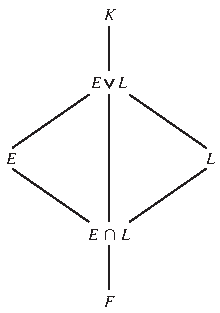
\includegraphics[width=0.301\linewidth,height=.8\textheight,keepaspectratio]{assets/p388_20.pdf}\end{center}
\begin{center}\small\textbf{46.13 Figure}\end{center}
\end{BookFloat}

\end{BookBody}
\ifdefined\BookMaster\let\BookFinish\relax\else\def\BookFinish{\end{document}}\fi\BookFinish
